\subsection{Sun Scan}
We performed sun scans with two different settings.
A step size of \SI{0.5}{\degree} with a total scan width of \SI{20}{\degree} and a step size of \SI{0.1}{\degree} with a total scan width of \SI{10}{\degree}.
For each of the settings we performed a horizontal and a vertical scan centered around the sun.
The integrated power spectra are then each normalized by subtracting the minimum and then dividing with the (new) maximum.
These normalized values are shown in figure~\ref{fig:sun_scan}

\begin{figure}[H]
    \centering
    \begin{subfigure}[t]{0.45\linewidth}
        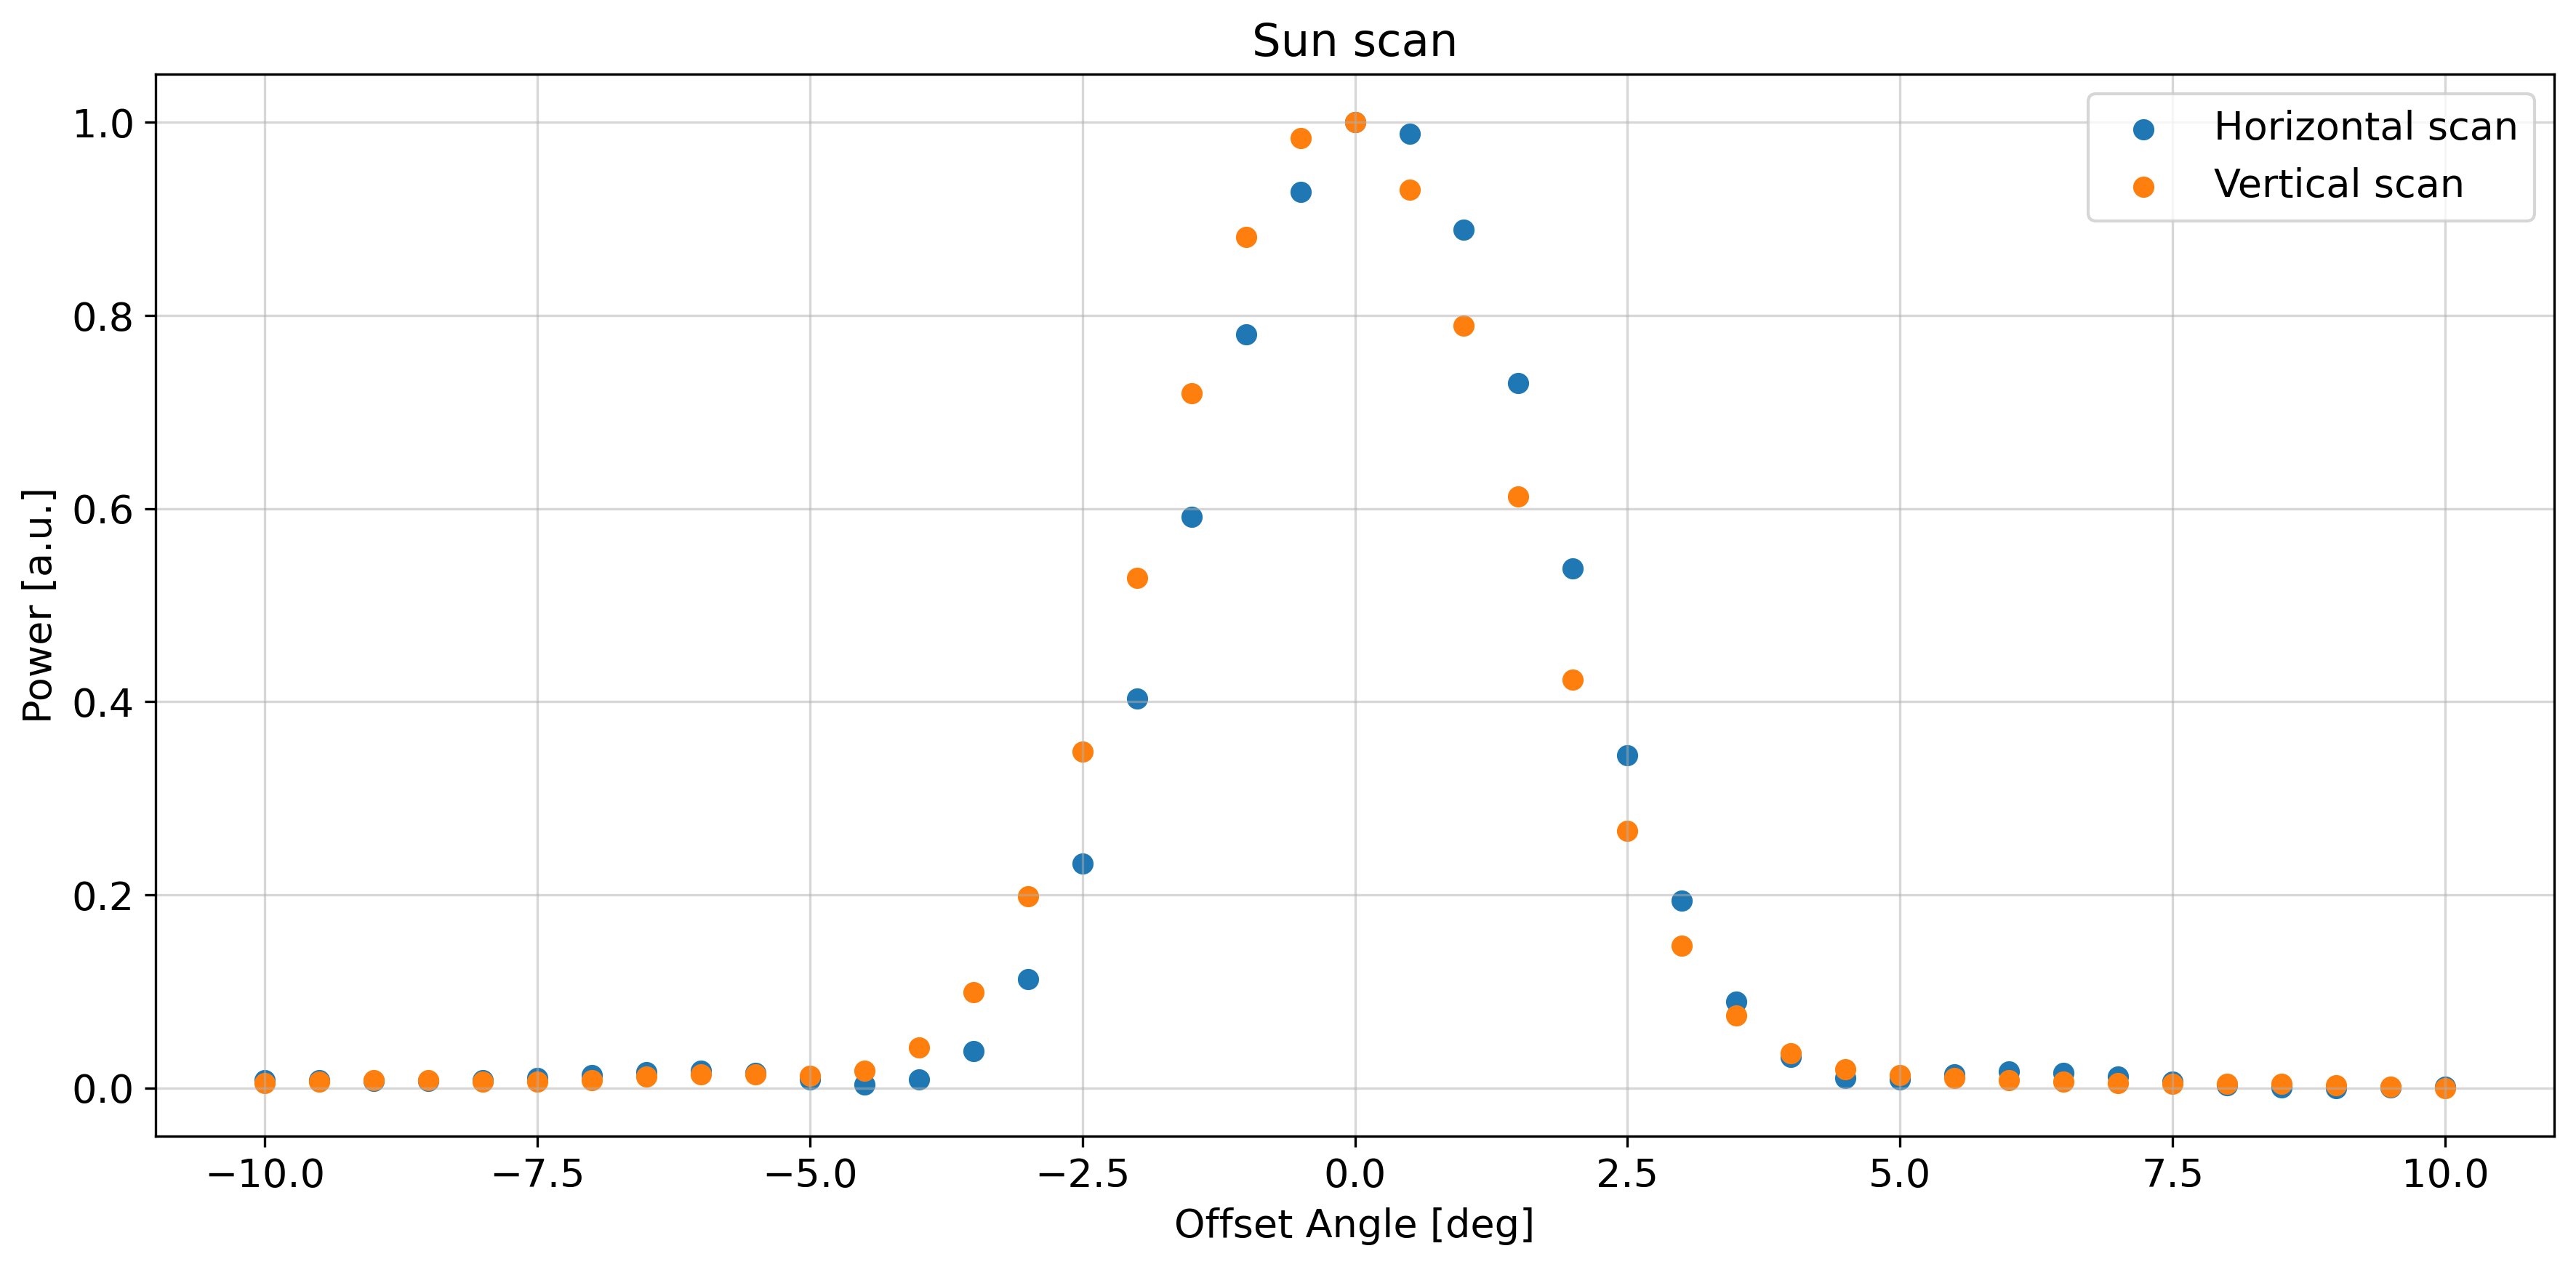
\includegraphics[width=\linewidth]{assets/sun_scan_low_res.png}
    \end{subfigure}
    \begin{subfigure}[t]{0.45\linewidth}
        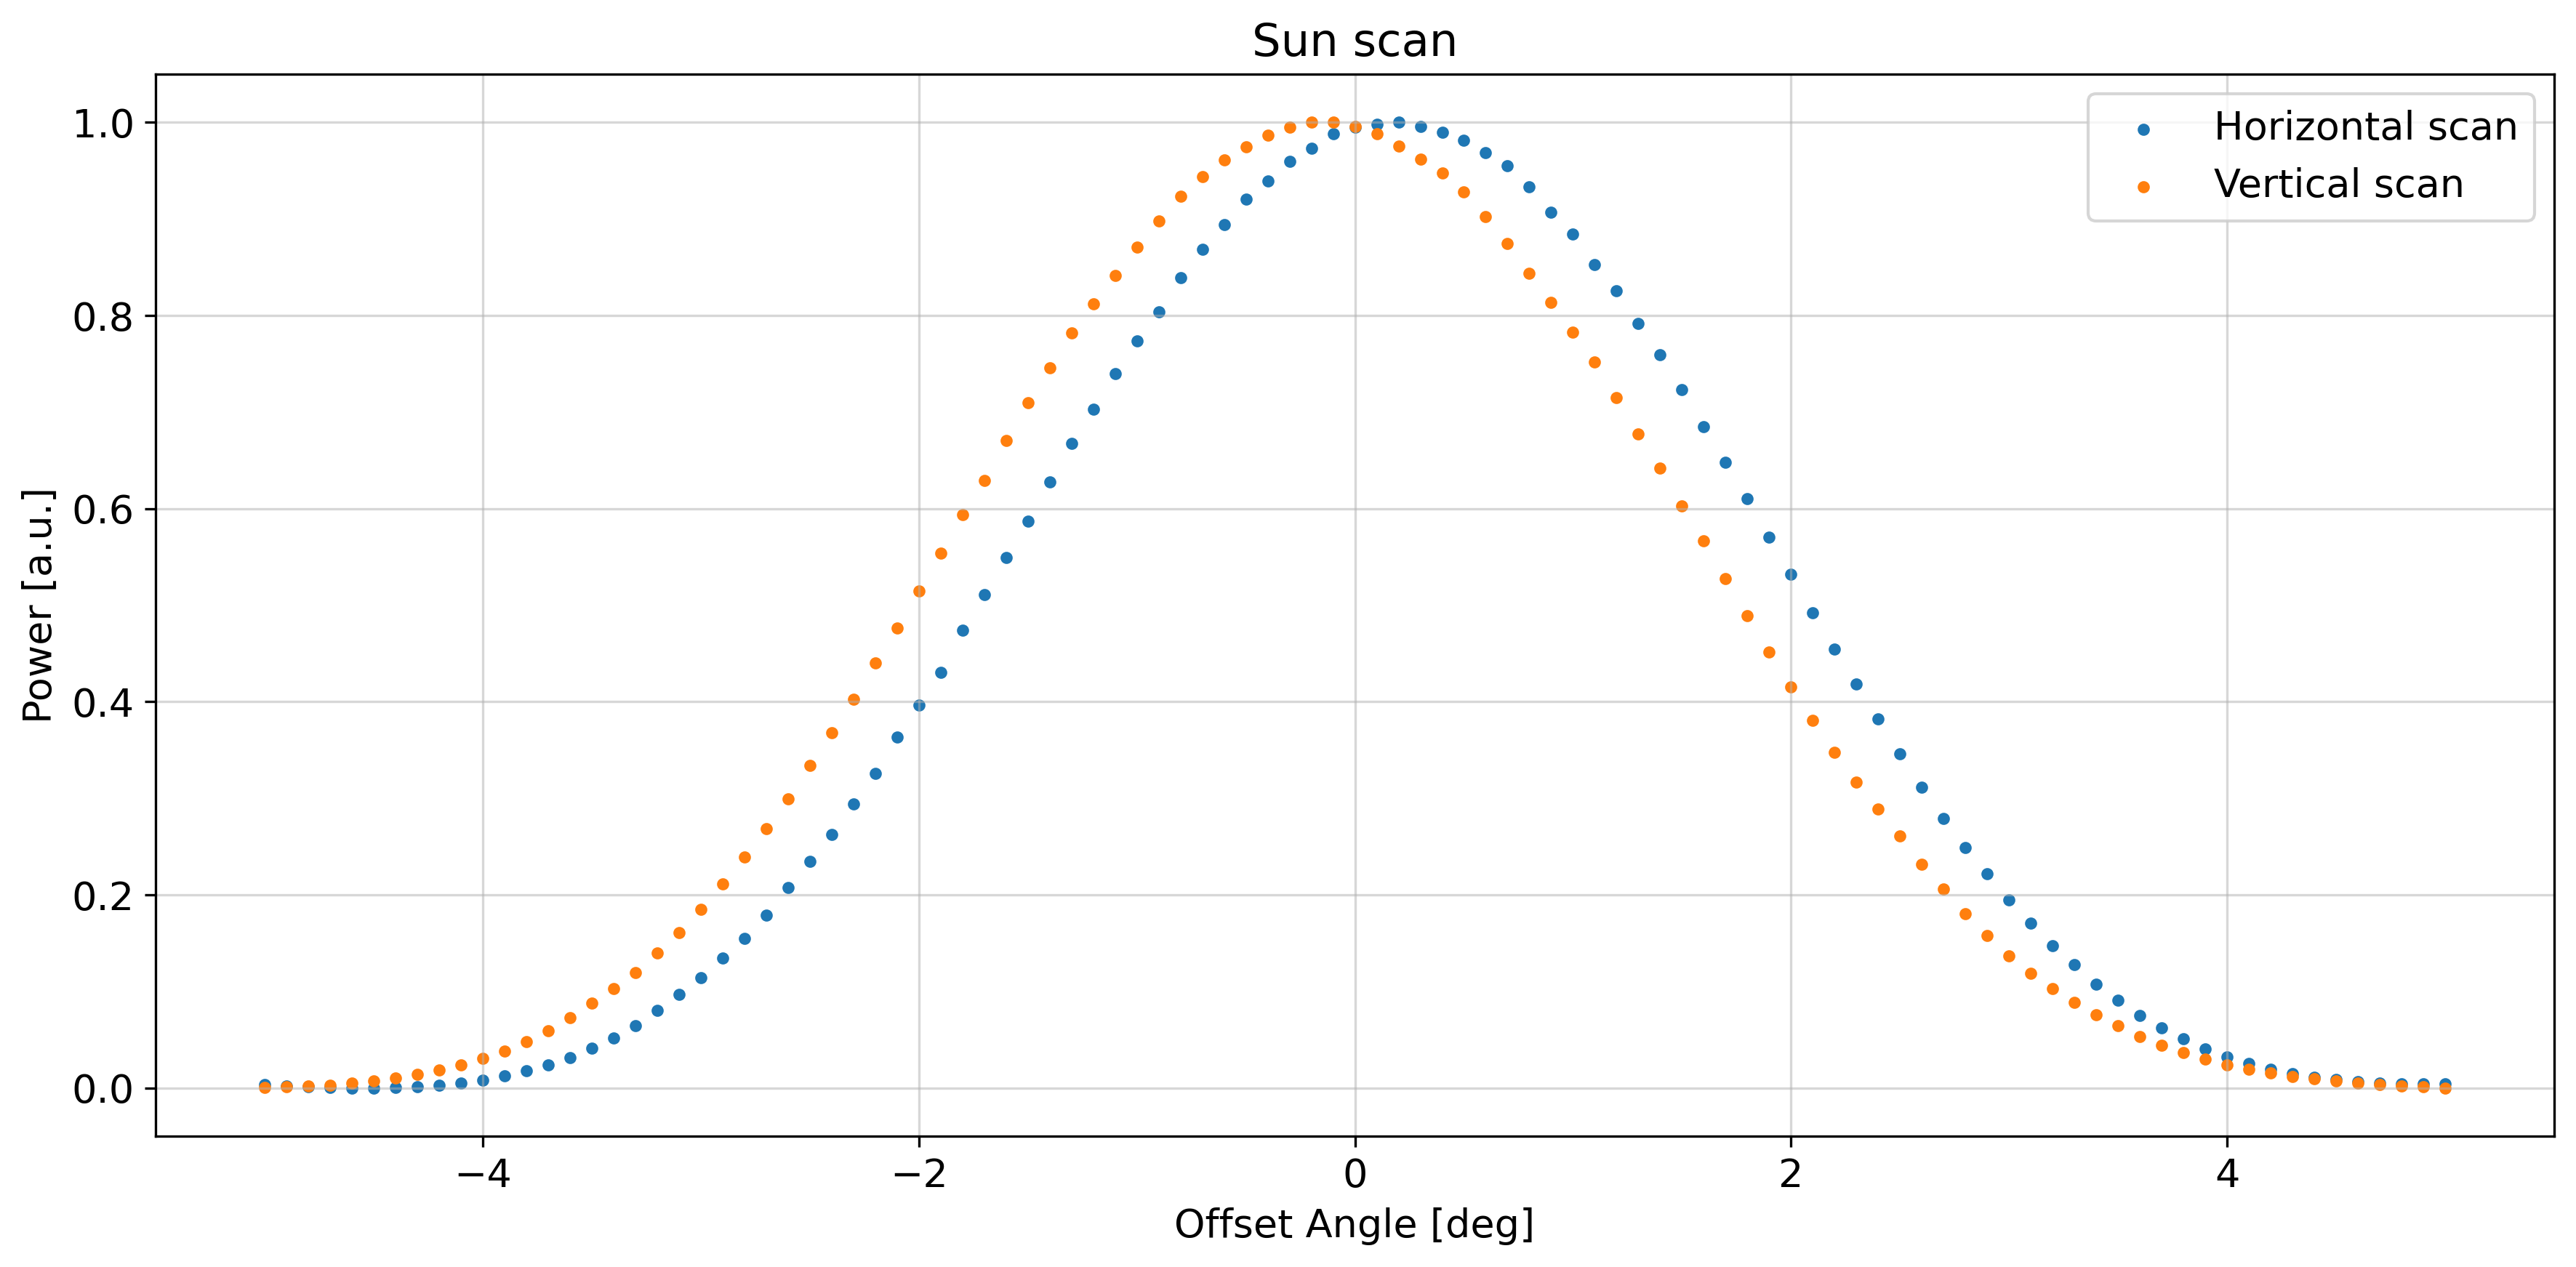
\includegraphics[width=\linewidth]{assets/sun_scan_high_res.png}
    \end{subfigure}
    \caption{Scan of the sun}
    \label{fig:sun_scan}
\end{figure}

The side bulbs are more visible when the normalizes power is shown logarithmically, this is shown in figure~\ref{fig:sun_scan_log}
\begin{figure}[H]
    \centering
    \begin{subfigure}[t]{0.45\linewidth}
        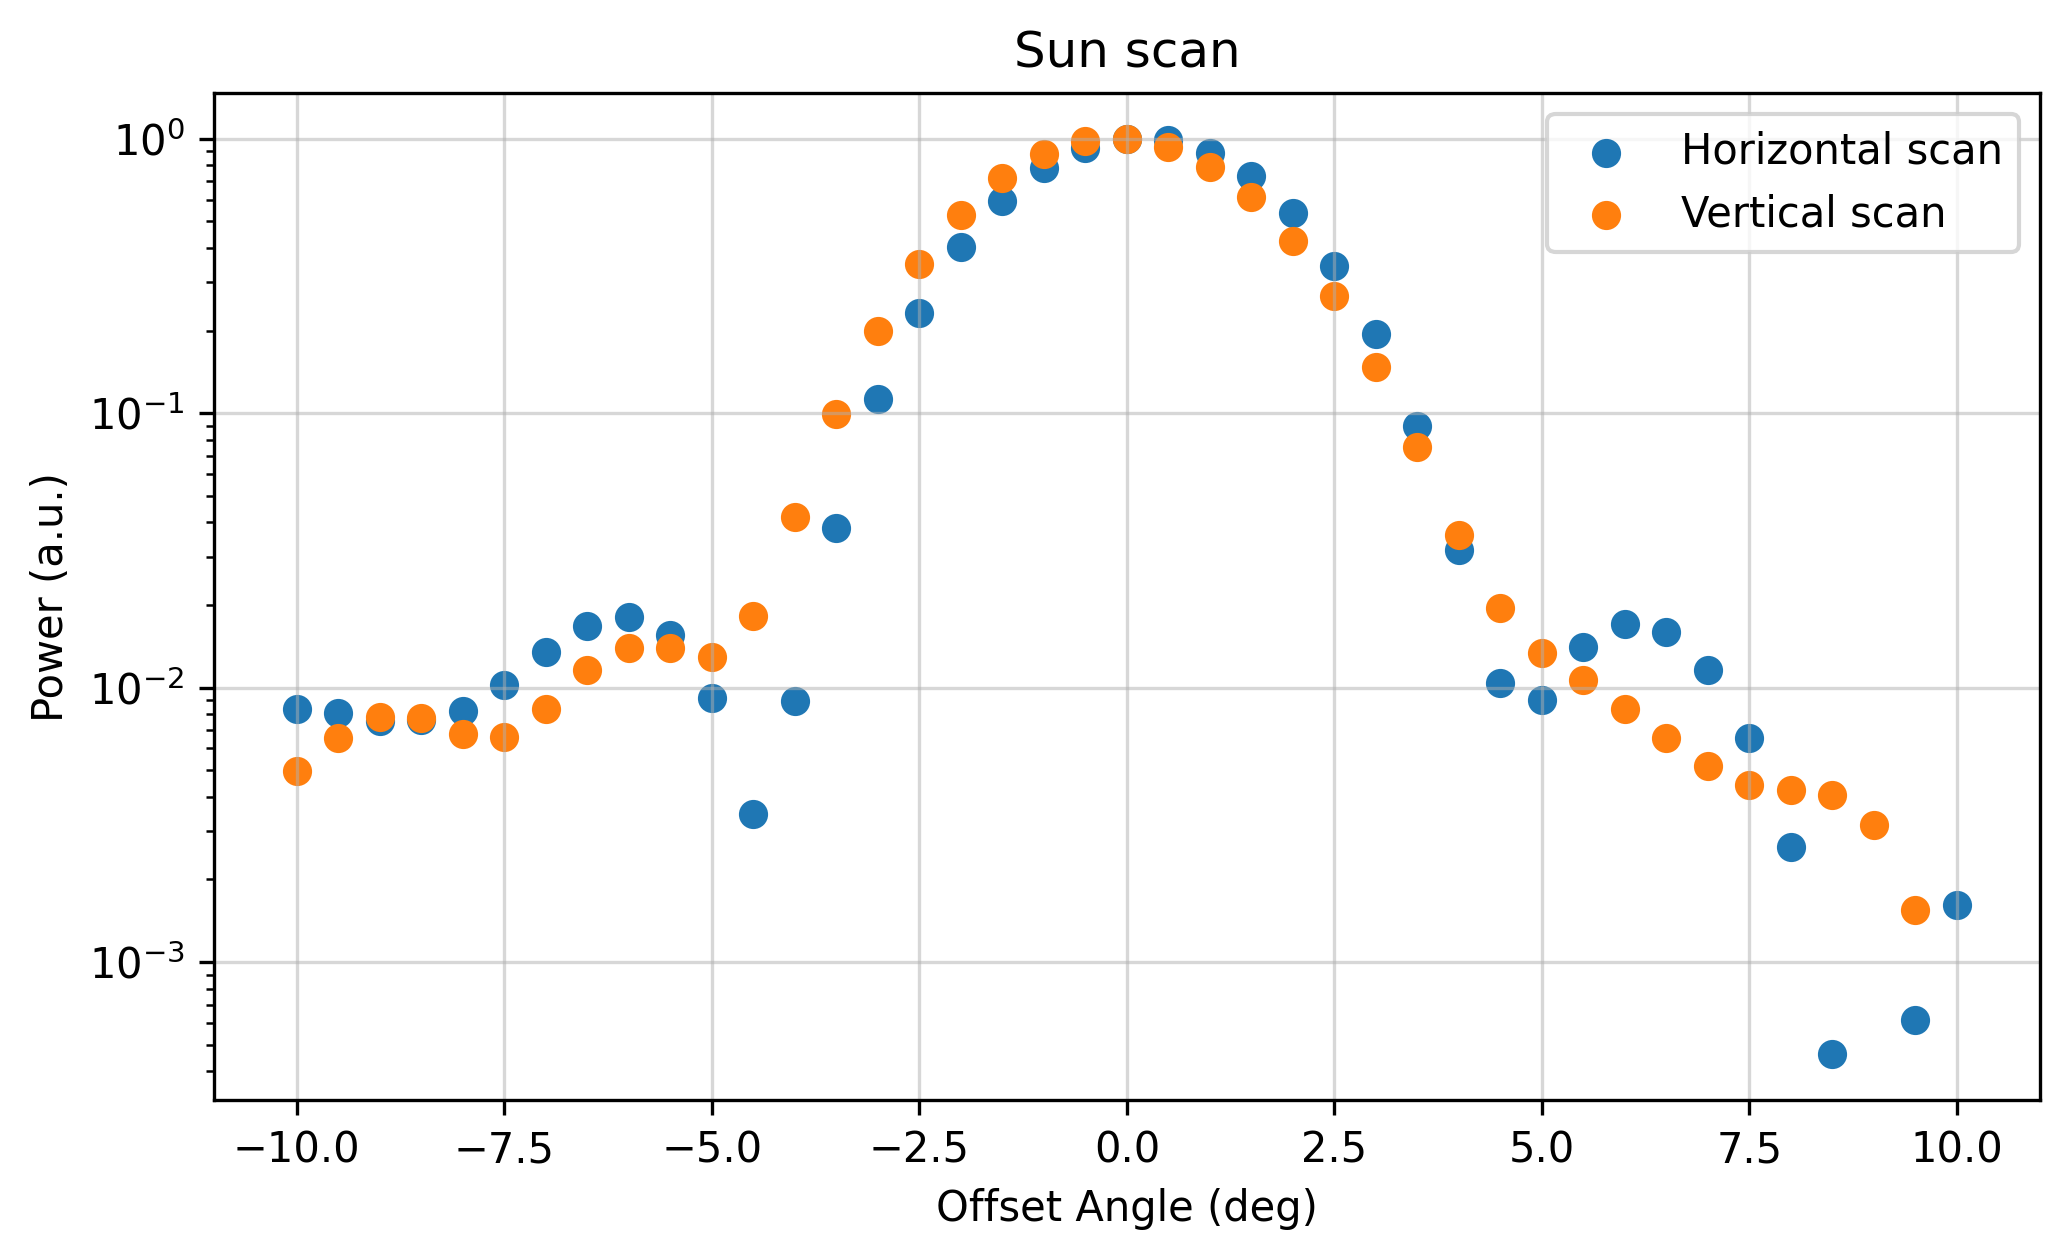
\includegraphics[width=\linewidth]{assets/sun_scan_low_res_log.png}
    \end{subfigure}
    \begin{subfigure}[t]{0.45\linewidth}
        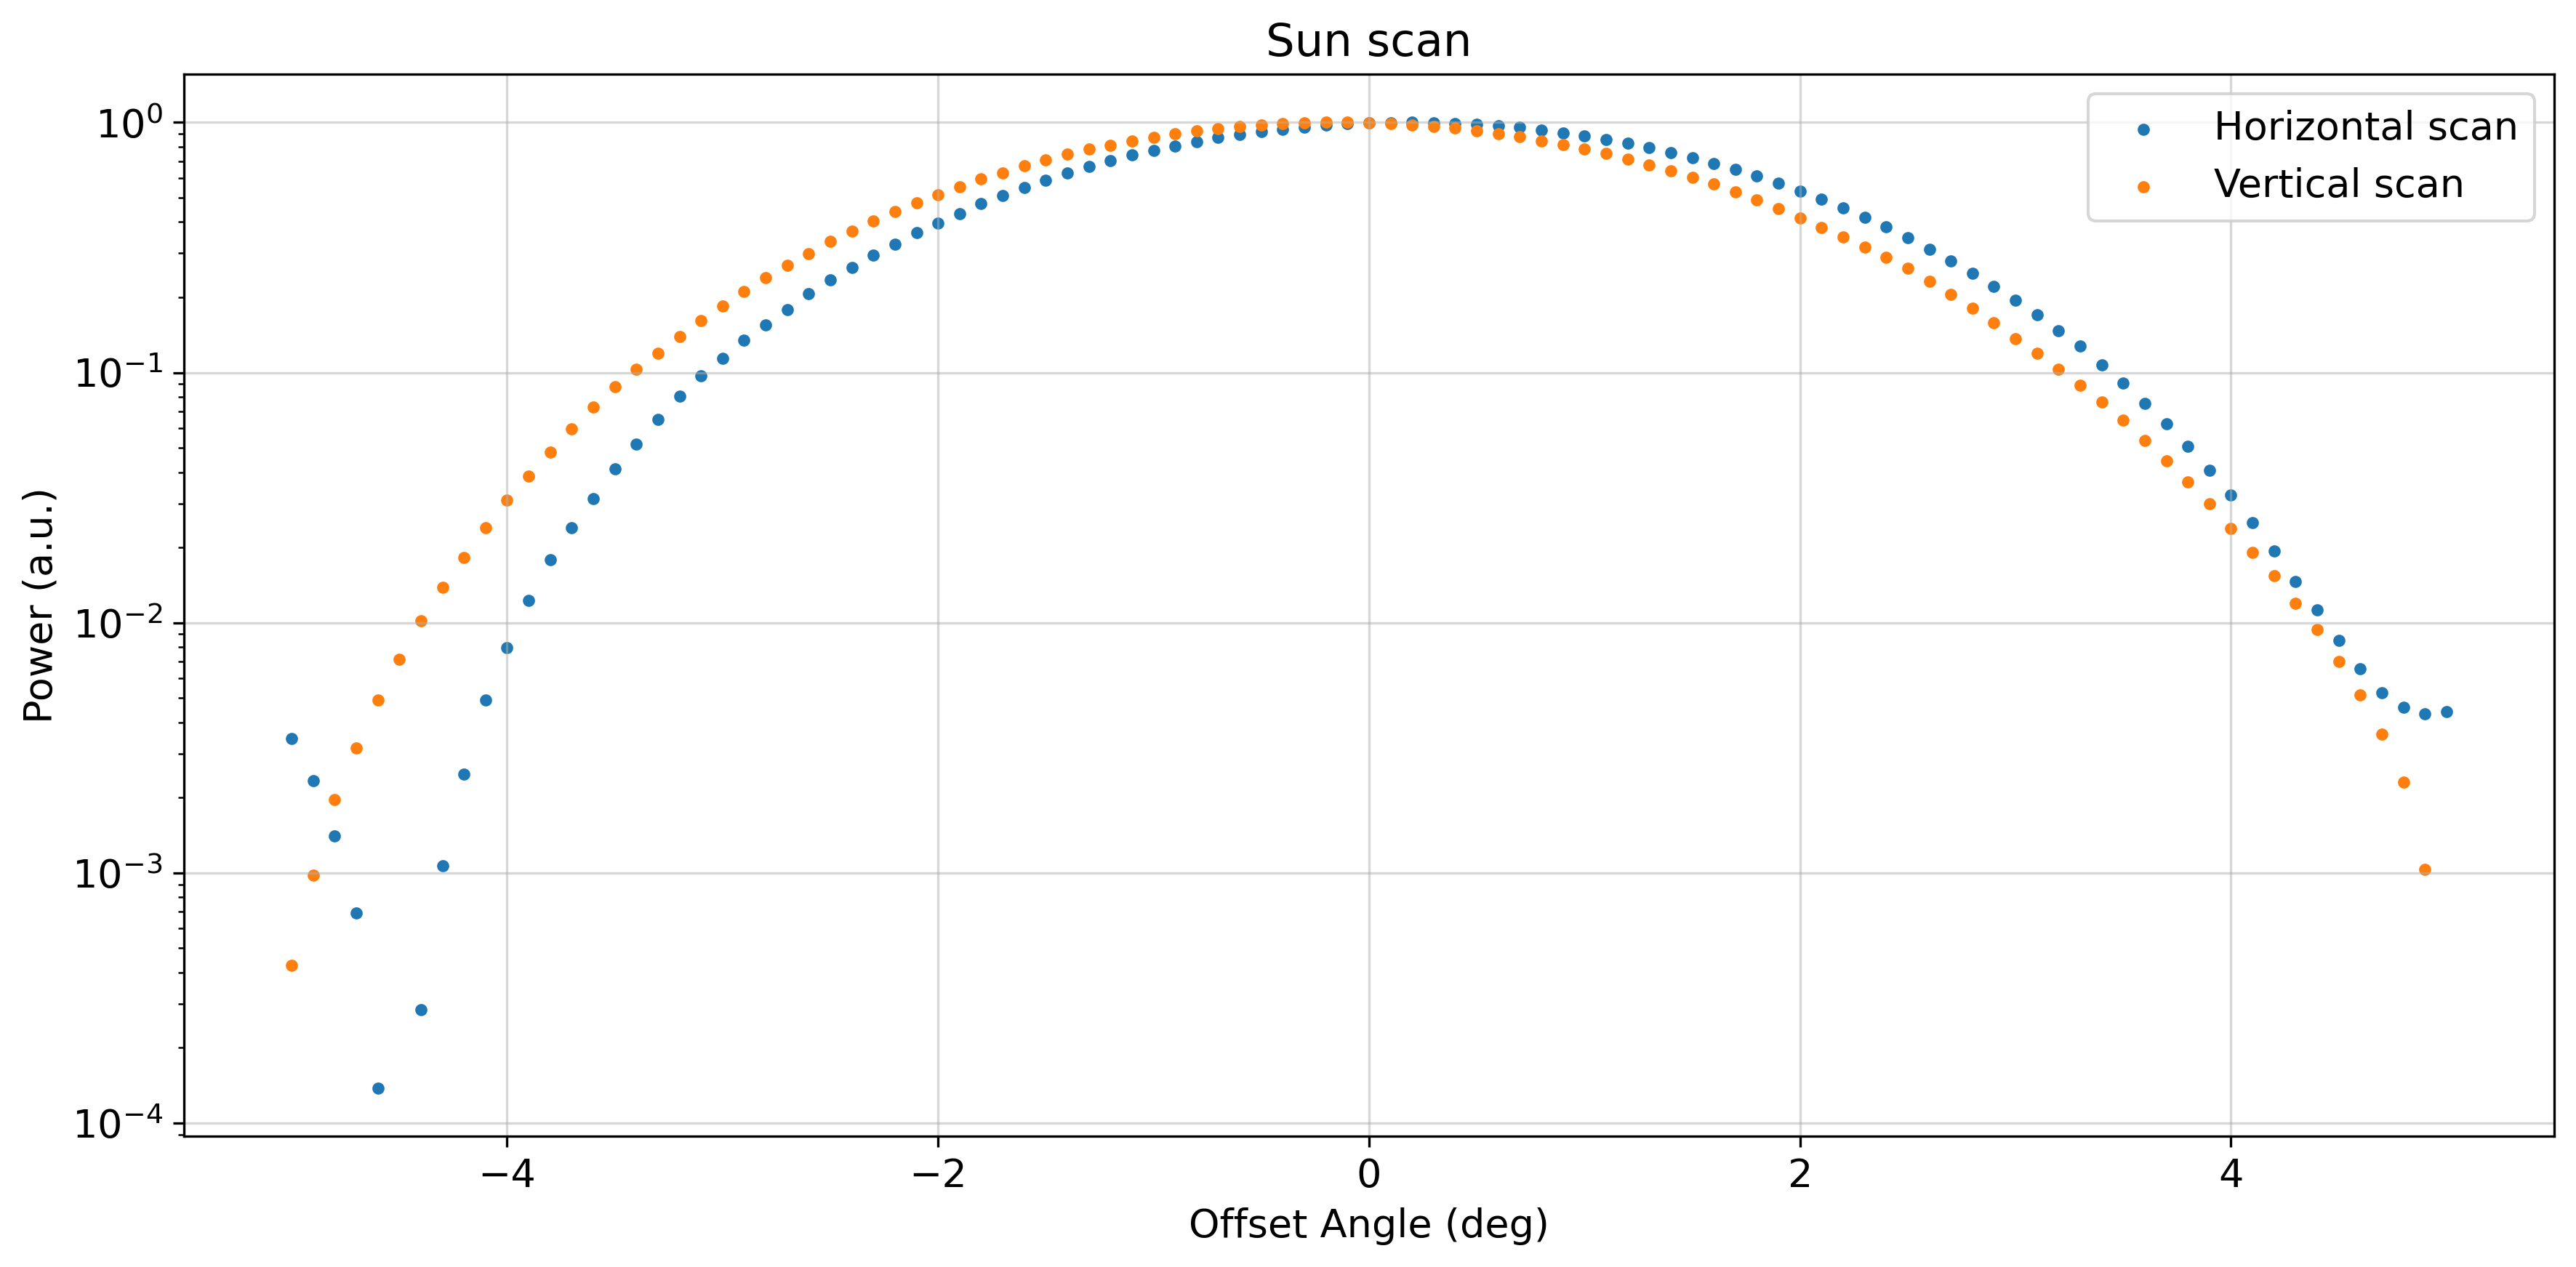
\includegraphics[width=\linewidth]{assets/sun_scan_high_res_log.png}
    \end{subfigure}
    \caption{Scan of the sun with logarithmic scale}
    \label{fig:sun_scan_log}
\end{figure}

To determine the full width at half maximum (FWHM) we use the high resolution data and fit it to a gaussian.
The equation describing the functional model is
\begin{equation}
    f(\theta)_{\theta_0\;\sigma} = \exp{\left(-\frac{(\theta-\theta_0)^2}{2\sigma^2}\right)}
\end{equation}.
The model can then be fitted using iterative least squares as described in \cite{adj_comp}. The FWHM can then be computed using \eqref{eq:FWHM}.
The resulting values are shown in table \ref{tab:params} and figure \ref{fig:sun_scan_fit}.
\begin{table}[H]
    \centering
    \begin{tabular}{lrrr}
        \toprule
        Direction & FWHM [\si{\degree}]& $ \sigma$ [\si{\degree}] & $ \theta_0 $ [\si{\degree}]\\
        \midrule
        Horizontal & \num{3.720(0.010)} & \num{1.581(0.005)} & \num{0.179(0.006)} \\
        Vertical & \num{3.751(0.009)} & \num{1.593(0.004)} & \num{-0.131(0.005)} \\
        \bottomrule
    \end{tabular}
    \caption{functional model parameters from least squares fit}
    \label{tab:params}
\end{table}
\begin{figure}[H]
    \centering
    \begin{subfigure}[b]{0.45\textwidth}
        \centering
        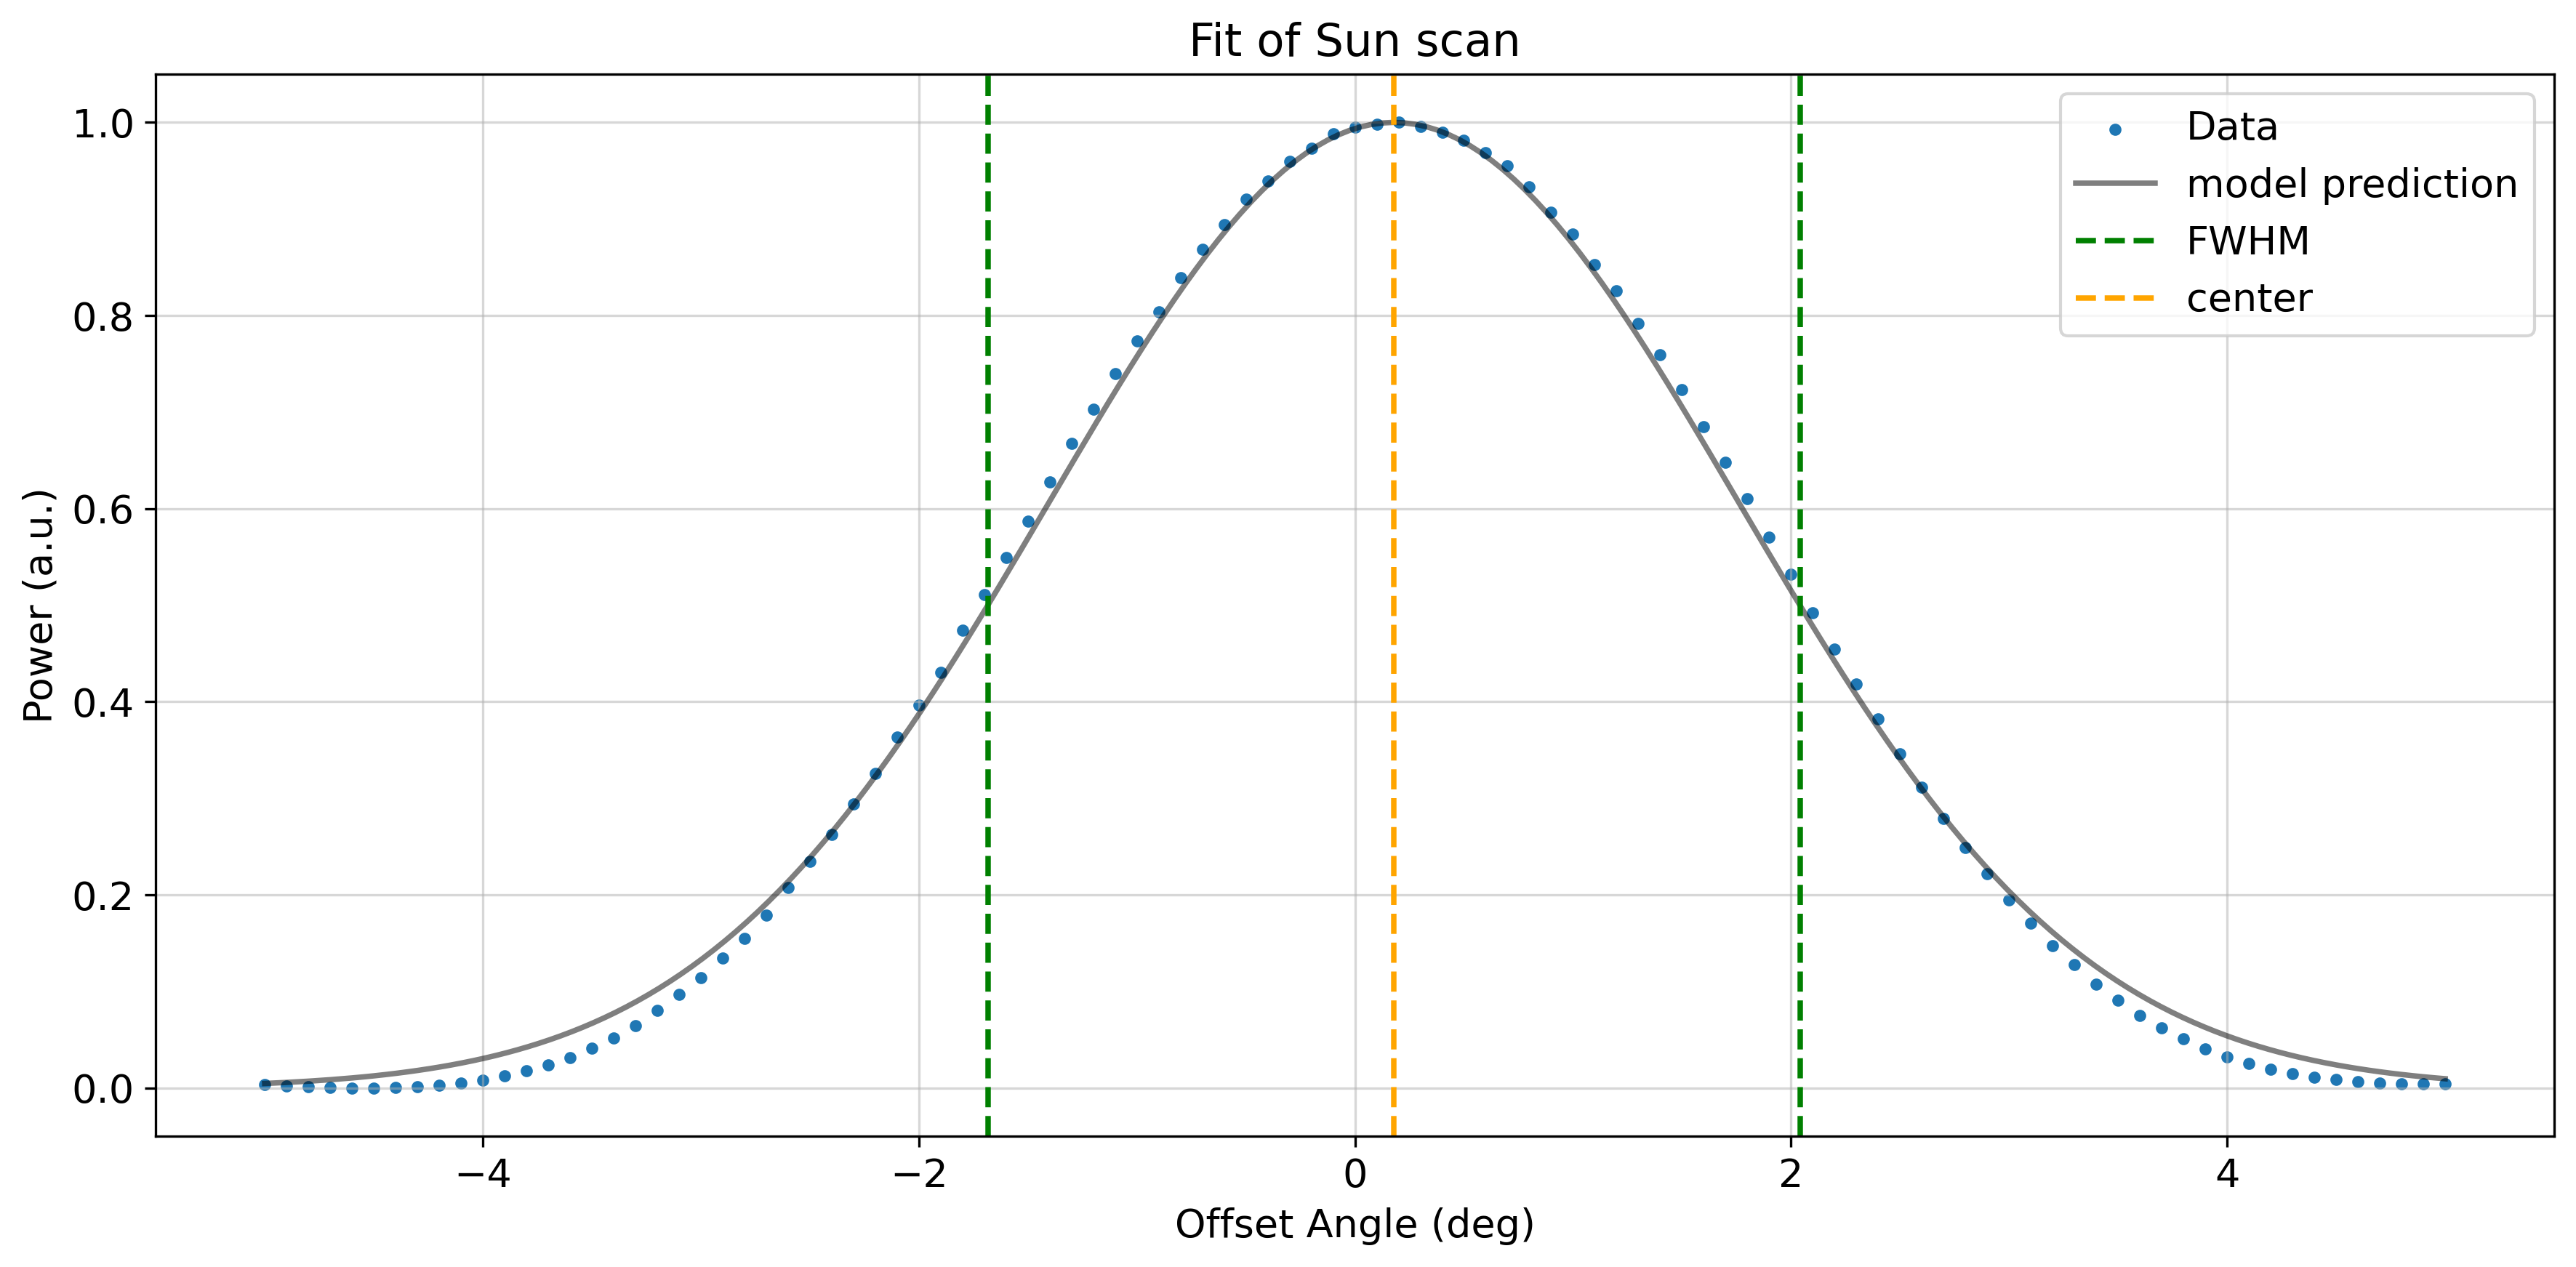
\includegraphics[width=\textwidth]{assets/sun_scan_fit_h.png}
        \caption{Fit to the horizontal scan}
        \label{fig:sun_fit_h}
    \end{subfigure}
    \hfill
    \begin{subfigure}[b]{0.45\textwidth}
        \centering
        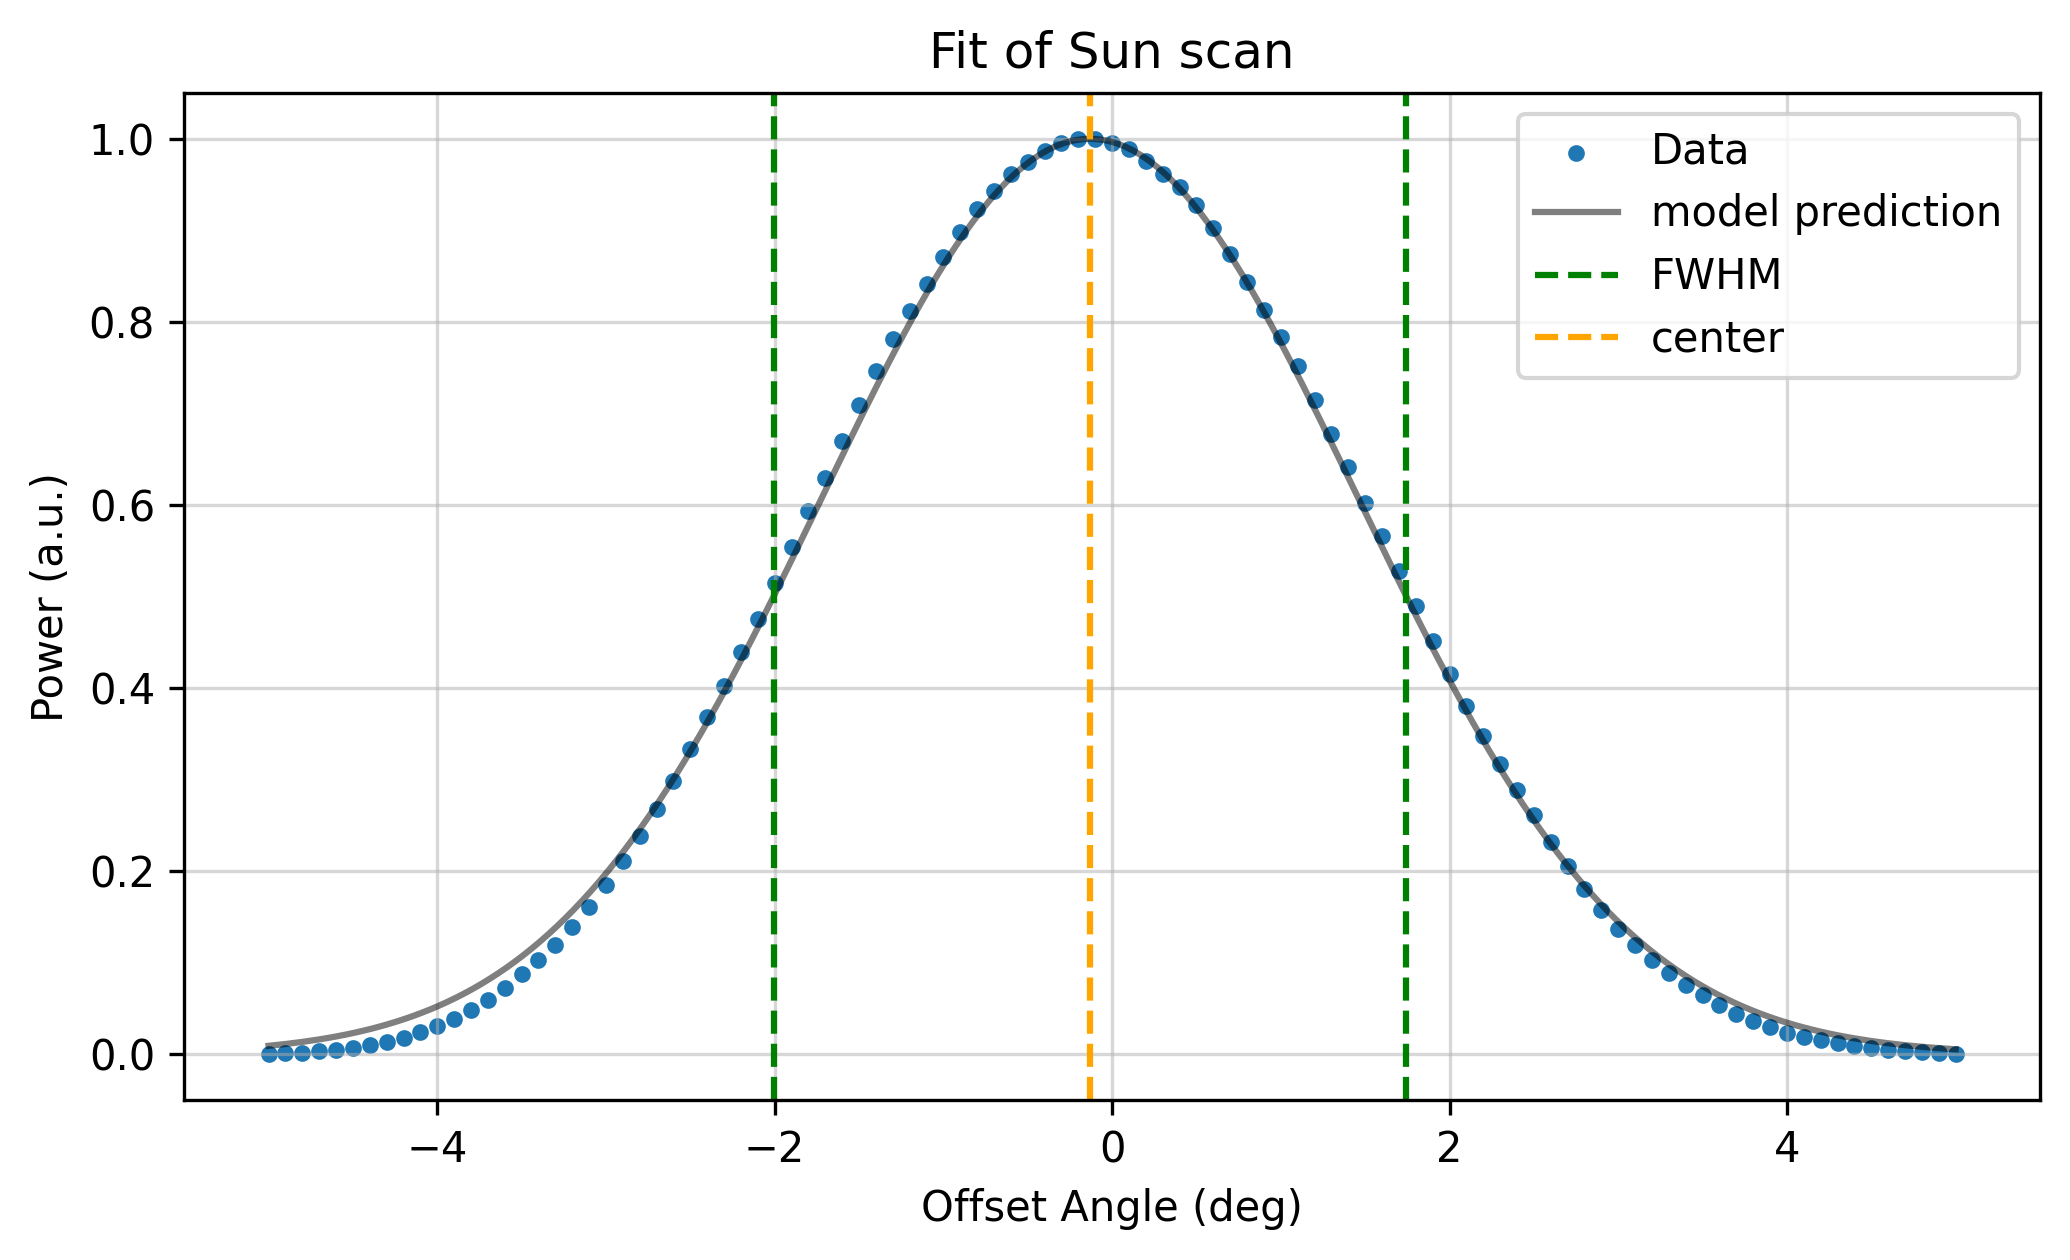
\includegraphics[width=\textwidth]{assets/sun_scan_fit_v.png}
        \caption{Fit to the vertical scan}
        \label{fig:sun_fit_v}
    \end{subfigure}
    \caption{Iterative least squares fits to the sun scans}
    \label{fig:sun_scan_fit}
\end{figure}
If we compare the values for the FWHM from table \ref{tab:params} with those from table \ref{tab:ang_res}
we find that the theoretical values do not lie withing the error bounds of the measured value.
We think the reason for this discrepancy is a combination of
\begin{itemize}
    \item Unknown errors in the given constants $d = \SI{4}{m}$ and $\eta = 0.5$, especially $\eta$ since it is not trivial to measure.
    \item Invalid assumption that the main bulb is gaussian.
    \item Invalid assumption that the solid angle that is not in the main bulb is negligible.
    \item Invalid assumption that the contribution from the integral in \eqref{eq:gauss_integral} of the gaussian with $\theta > \pi$ is negligible.
\end{itemize}
Of these we think that the uncertainty in $\eta$ has the biggest contribution to the error.